\chapter{Implémentation}
\label{chap:impl}

\section{Introduction}
Dans le chapitre précédent, nous avons généralement présenté des méthodes concernant notre travail. Après avoir étudié des différentes méthodes, dans chaque étape, nous avons choisi une méthode qui peut mieux adapter à notre travail. Durant notre recherche, il existe déjà des codages qui a la performance efficace, donc, nous avons réutilisé ces codages. Au contrait, pour les étapes qui existent pas encore des codages, nous avons les implémenté nous-même ou nous avons modifié des codages qui n'ont bien adapté pas à notre travail.

\section{Représentation par des descripteurs et méthode sac de mots}
La description des images est une méthode très importante dans la classification des images. Cette étape est beaucoup influencée au résultat final. Dans le domaine de recherche d'images et de classification d'images, le descripteur SIFT \cite{low04} est un caractéristique important pour la représentation des images. Cette méthode est de plus en plus populaire. A partir de l'idée de la classification des texte, dans la recherche en 2007 \cite{bos07}, les auteurs proposent un système de classification d'images utilisant le descripteur SIFT et le modèle sac de mot (Bag of Visual Word). Cette méthode peut diviser en 3 étapes :
\begin{enumerate}
\item trouver des descripteurs locales des images (des caractères)
\item construire un dictionnaire a partir des caractères
\item représenter des images par des histogrammes
\end{enumerate}

Dans ces étapes, nous avons réutilisé des codages existant en modifiant des entrées et des sorties pour adapter aux étapes suivantes. Précisément, dans l'étape \textit{1}, nous avons réutilisé le codage de D.Lowe \cite{low99} pour créer des vecteurs de caractéristiques (descripteurs). Ensuite, l'étape \textit{2} sert à construire un dictionnaire. Dans cette étape, la méthode k-moyenne \cite{mq67} est appliquée afin de créer des clusters a partir des vecteurs SIFT créés dans l'étape \textit{1}. L'ensemble de clusters est considéré comme un dictionnaire. Enfin, dans l'étape \textit{3}, une image est représentée par un histogramme. Dans cette étape, d'abord, on met chaque vecteur SIFT dans chaque image à un cluster le plus proche de ce vecteur (sa base sur la distance entre ce vecteur au centre des clusters). Ensuite, on compte le fréquence des mots d'une image existe dans le dictionnaire créé dans l'étape \textit{2} pour représenter l'image comme un histogramme de fréquence. Pour l'étape \textit{3}, nous avons implémenté en C/C++.

\section{Apprentissage automatique}
Avec notre processus, après la méthode sac de mot visuel, nous appliquons un algorithme d'apprentissage pour classifier des images vers leurs classes. Nous avons développé la méthode MC-SGD et pour vérifier la performance de notre méthode, nous avons fait la comparaison avec l'application LIBSVM \cite{cl01}, l'implémentation de SVM le plus utilisée actuellement.

\subsection{Descente de gradient stochastique (SGD)}
Pour cette méthode, il existe plusieurs d'implémentations différentes. Dans notre travail, nous avons réutilisé l'implémentation \textit{Pegasos} \cite{sss07} ci-dessous :

\begin{algorithm}
\caption{L'algorithm d'apprentissage SGD-SVM binaire}\label{sgdal}
\begin{algorithmic}[1]
\Procedure{trainBinaireSGDSVM}{$D$, $y$, $\lambda$, $T$, $n$}

\State Initialiser $w_1 = 0$

\For{\texttt{t = 0; t < T; t++}}

\State $\eta = \frac{1}{\lambda}$

\Comment{Boucle pour choisir ex exemples chaque cycle}
\For{\texttt{ex = 0; ex < n; ex++}}
\State \texttt{choisir un exemple aléatoire dans D}
\If{\texttt{${y_i}_t.(w_t,{x_i}_t) < 1$}}
\State $w_{t+1} = (1 - \eta_t.\lambda).w_t + \eta_t.{y_i}_t.{x_i}_t$
\Else
\State $w_{t+1} = (1 - \eta_t.\lambda).w_t$
\EndIf
\EndFor

\EndFor

\State Return $w_{t}$

\EndProcedure
\end{algorithmic}
\end{algorithm}


\pagebreak
\subsection{Descente de gradient stochastique pour multi-classe (MC-SGD)}
Comme les autres algorithme de SVM, SGD est implémenté pour résoudre le problème de classification de 2 classes. L'implémentation \textit{Pegasos} \cite{sss07} est efficace. A partir de cette implémentation, nous les avons modifié et développé pour résoudre le problème de multi-classes (k classes, $k \geq 3$). \\

Pour le problème de classification de multi-classes, comme nous avons expliqué dans la partie précédente, nous avons utilisé la méthode \textit{one-vs-all}. Cette méthode ne construit que k classificateur (k est le nombre de classes). Par exemple, quand le problème a trois classes comme l'image \ref{mclass}. \textit{One-vs-all} va construire trois classificateurs comme l'image \ref{1vsall}.

\pagebreak
\begin{figure}
        \centering
        \begin{subfigure}[b]{0.5\textwidth}
                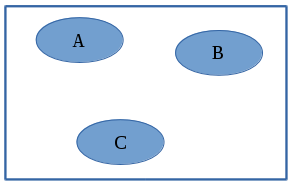
\includegraphics[width=\textwidth]{images/multiclass}
                \caption{Problème}
                \label{mclass}
        \end{subfigure}%
        ~ %add desired spacing between images, e. g. ~, \quad, \qquad, \hfill etc.
          %(or a blank line to force the subfigure onto a new line)
        \begin{subfigure}[b]{0.5\textwidth}
                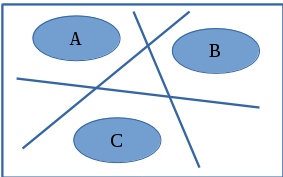
\includegraphics[width=\textwidth]{images/mlclass}
                \caption{one-vs-all}
                \label{1vsall}
        \end{subfigure}
        \caption{Problème de multi-classes}\label{mulclass}
\end{figure}


L'image \ref{1vsall} est comme un résumé de one-vs-all. Pour plus claire, nous vous listons les trois classificateurs de ces trois classes comme l'image \ref{1vsalldetail}

\begin{figure}
        \centering
        \begin{subfigure}[b]{0.3\textwidth}
                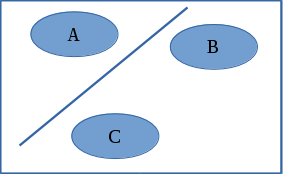
\includegraphics[width=\textwidth]{images/classa}
                \caption{classe A}
                \label{classa}
        \end{subfigure}%
        ~ %add desired spacing between images, e. g. ~, \quad, \qquad, \hfill etc.
          %(or a blank line to force the subfigure onto a new line)
        \begin{subfigure}[b]{0.3\textwidth}
                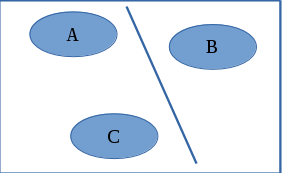
\includegraphics[width=\textwidth]{images/classb}
                \caption{class B}
                \label{classb}
        \end{subfigure}
        ~ %add desired spacing between images, e. g. ~, \quad, \qquad, \hfill etc.
          %(or a blank line to force the subfigure onto a new line)
        \begin{subfigure}[b]{0.30\textwidth}
                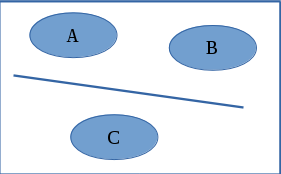
\includegraphics[width=\textwidth]{images/classc}
                \caption{class C}
                \label{classc}
        \end{subfigure}
        \caption{Problème de multi-classes}\label{1vsalldetail}
\end{figure}




\makeatletter
\def\BState{\State\hskip-\ALG@thistlm}
\makeatother


\begin{algorithm}
\caption{L'algorithm d'apprentissage SGD-SVM pour multi-classes}\label{mcsgdal}
\begin{algorithmic}[1]
\Procedure{trainMCSGDSVM}{$D$, $y$, $k$, $\lambda$, $T$, $n$}

\Comment{D est les données d'apprentissage }\\
\Comment{y est les labels des données }\\
\Comment{k est le nombre de classes dans D}\\
\Comment{$\lambda$ est le constant possible }\\
\Comment{T est le nombre de cycles }\\
\Comment{n est le nombre d'exemple par cycle }\\

\State Initialiser k modèles w

\For{\texttt{c = 0; c < k; c++}}\\
\Comment{Préparation des données pour one-vs-all}
\State \texttt{$y_i = +1$ si l'exemple de classe c, $y_i = -1$ sinon}
\State \texttt{$w_c = trainBinaireSGDSVM(D, y, \lambda, T, n)$} $(c-vs-all)$
\EndFor

\State Return $w$

\EndProcedure
\end{algorithmic}
\end{algorithm}

\pagebreak
\subsection{Parallélisation de MC-SGD}
Nous trouvons que l'algorithme \ref{mcsgdal} linaire, il apprend les modèles l'un après l'autre sur un seul cœur du processeur d'ordinateur. Donc, les autres cœurs ne font rien et l'algorithme est lent. A notre époque, nous pouvons utiliser tous les cœurs possibles pour améliorer la vitesse de notre algorithme en utilisant la programmation parallèle.\\

Pour le problème de multi-classes (k classes), l'algorithme SGD-SVM apprend indépendant chaque classificateur. Donc, c'est possible d'apprendre chaque classificateur sur chaque cœur différent. Dans notre implémentation, nous avons parallélisé la boucle sur l'apprentissage des classificateur. Supposons que nous avons p processeurs et k classificateurs. Donc, chaque processeur apprend $n = \frac{k}{p}$ ou $n = \frac{k}{p} + 1$ classificateurs.

\pagebreak
\begin{algorithm}
\caption{L'algorithm d'apprentissage SGD-SVM parallèle pour multi-classes}\label{pmcsgdal}
\begin{algorithmic}[1]
\Procedure{trainMCSGDSVMParallel}{$D$, $y$, $k$, $\lambda$, $T$, $n$}

\State Initialiser k modèles w
\\
\BState \textbf{Pocesseur 1:}
\State \texttt{$y_i = +1$ si l'exemple de classe c (c = 1, classe 1.p + 1, classe 2.p + 1, ...) et $y_i = -1$ sinon}
\State \texttt{$w_c = trainBinaireSGDSVM(D, y, \lambda, T, n)$} $(c-vs-all)$
\\
\BState \textbf{Pocesseur 2:}
\State \texttt{$y_i = +1$ si l'exemple de classe c (c = 2, classe 1.p + 2, classe 2.p + 2, ...) et $y_i = -1$ sinon}
\State \texttt{$w_c = trainBinaireSGDSVM(D, y, \lambda, T, n)$} $(c-vs-all)$

\State .
\State .
\State .
\\
\BState \textbf{Pocesseur p:}
\State \texttt{$y_i = +1$ si l'exemple de classe c (c = p, classe 1.p + p, classe 2.p + p, ...) et $y_i = -1$ sinon}
\State \texttt{$w_c = trainBinaireSGDSVM(D, y, \lambda, T, n)$} $(c-vs-all)$

\BState Return $w$

\EndProcedure
\end{algorithmic}
\end{algorithm}

Avec la structure comme l'algorithme \ref{pmcsgdal}, à chaque boucle, p processeurs apprennent p classificateurs en parallèle. Alors, la vitesse améliore presque p fois si l'on compare avec la version linaire de cet algorithme, l'algorithme \ref{mcsgdal}.


